\documentclass[11pt]{report}
\usepackage[margin=1.25in]{geometry}
\usepackage{graphicx,float}

%Biblatex
\usepackage[backend=biber,style=numeric]{biblatex}
\addbibresource{bibtex.bib}

% Figures
\usepackage{amsmath,amsthm,amsfonts}
\usepackage{rotating}
\usepackage{subcaption} % For side-by-side figures

% For labelings/struct descriptions
\usepackage{blindtext}
\usepackage{scrextend}
\addtokomafont{labelinglabel}{\sffamily}

\usepackage{listings} % For source code
\usepackage{algorithm,algorithmicx,algpseudocode} % For algorithms

% Commands
\newcommand{\abs}[1]{\left|#1\right|}
\newcommand{\dist}[2]{\text{dist}\left({#1, #2}\right)}
\newcommand{\leftc}[1]{\text{left child}\left(#1\right)}
\newcommand{\rightc}[1]{\text{right child}\left(#1\right)}

% Definitions, Theorems, and Corollaries
\newtheorem{defn}{Definition}[section]
\newtheorem{theorem}{Theorem}[section]
\newtheorem{corollary}{Corollary}[section]

%opening
\title{Graph Drawing Algorithms}
\author{Vincent La}

\begin{document}
    
\maketitle
\tableofcontents

\chapter{Introduction}
Graph theory is one of the most widely applicable fields of math, and as such there has been a large demand for different methods of visualizing graphs. Just as the types and uses of graphs are wide and varied, there are also a variety of different algorithms for visualizing graphs. These algorithms vary in the type of graphs they will draw, and the guarantees they may provide, e.g. planarity and symmetry. This paper will further explore some of the algorithms detailed by \textit{Graph Drawing: Algorithms for the Visualization of Graphs}. \cite[see][page 12]{Battista:1998:GDA:551884}

\bigskip

All proofs, and associated errors, are my own unless otherwise noted.

\section{Computer Science Basics}
Although this is a paper on applied math,\footnote{As the author claims} because it also focuses on the analysis of algorithms, some computer science fundamentals are required.
 
\subsection{Complexity}
When analyzing algorithms, one feature we want to analyze is how complicated they can get as the input size $n$ increases. For example, suppose we want to count the number of occurrences of 5 in an unsorted list. Because the list is unsorted, we do not know in general where the 5's are so we have to scan every item in the list. Hence, the running time $T(n)$ of this algorithm is based on the size of the list $n$ and we say this algorithm runs in in linear time.

\begin{defn}[$\Omega(f(n))$] We say an algorithm is $\Omega(f(n))$ if there is some positive constants $a, n_0$ such that $a \cdot f(n) \leq T(n)$ for all $n \geq n_0$.
\end{defn}

\begin{defn}[$O(f(n))$] We say an algorithm is $O(f(n))$ if there is some positive constants $b, n_0$ such that $b \cdot f(n) \geq T(n)$ for all $n \geq n_0$.
\end{defn}

\begin{defn}[$\Theta(f(n))$] We say an algorithm is $\Theta(f(n))$ if it is $\Omega(f(n))$ and $O(f(n))$.
\end{defn}

\subsubsection{What Gets Analyzed?}
Usually, algorithms are analyzed for their time complexity (how long it takes to compute something). However, they may also be analyzed for their space complexity (memory usage), and any other aspect of their performance. For example, with respect to graph drawing, algorithms may be analyzed for the amount of screen real estate they take up.

\chapter{Tree Drawing Algorithms}
\section{Motivation}
Many types of graphs are used in computer science, and one of the most common is the tree--especially binary trees. Binary trees--trees with at most two nodes--form the basis for many data structures in computer science. For example, when many people thinking of storing a collection of items to be searched later, the naive solution is to store them in a list. When checking to see if an item is part of this collection, a naive solution is to simply iterate through the list, comparing our item against each element of the list. In other words, for a collection of $n$ items, we have to perform $n$ comparisons.

\bigskip

However, a binary search tree is constructed such that for every node, every child node on its left is less than the value at the root, and vice versa for the right side. Hence, when searching for an item, if our item is less than the value at the current node, then we only need to keep searching in the left subtree. As a result, we can find an item we want with on average just $\log_2{n}$ comparisons. As a result of the many implementations of trees in computers, many have discussed ways of visualizing these data structures.

\begin{figure}[H]
    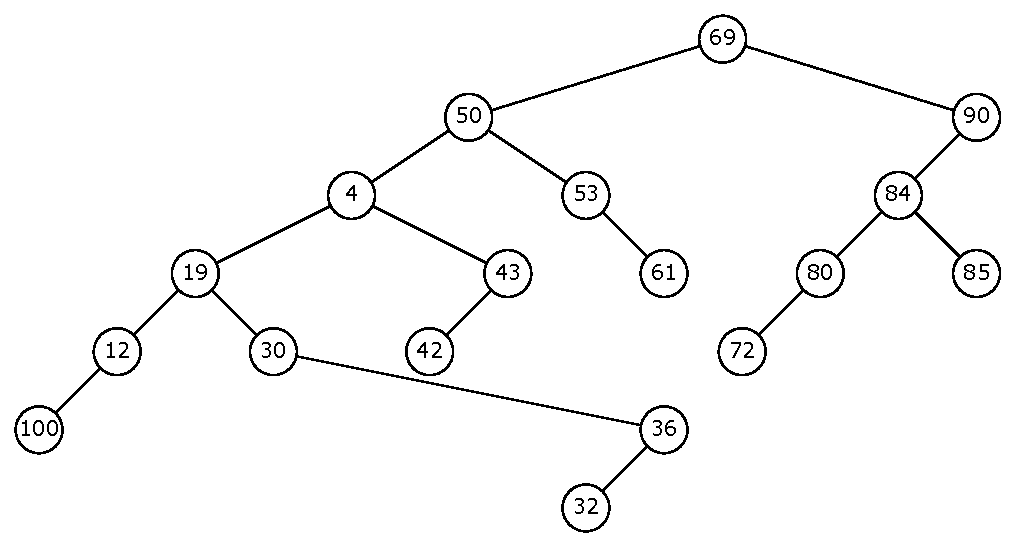
\includegraphics[width=\linewidth]{report/bst_20.pdf}
    \caption{A binary search tree with 20 items}
\end{figure}

\subsection{Definitions}
Before talking about trees, it would behoove us to build a common vocabulary about them.

\begin{defn}[Level (of a node)]
    The level (or depth) of a node in a binary tree is the number of edges between that node and the root. By convention, the root is on level 0.
\end{defn}

\begin{defn}[Height (of a tree)]
    The height of a binary tree is the number of edges between the root and the deepest leaf.
\end{defn}

\begin{defn}[Perfect Binary Tree]
    A perfect binary tree is a binary tree where all leaf nodes are on the same level, and all other nodes have two children.
\end{defn}

\subsubsection{Tree Traversal}
When implementing trees as computer data structures, there are a multitude of ways to traverse them.

\begin{defn}[Level Order Traversal]
    In a level order traversal, we move from top to bottom, left to right. In other words, a level order traversal is a breadth-first traversal of a tree.
\end{defn}

\begin{figure}[H]
    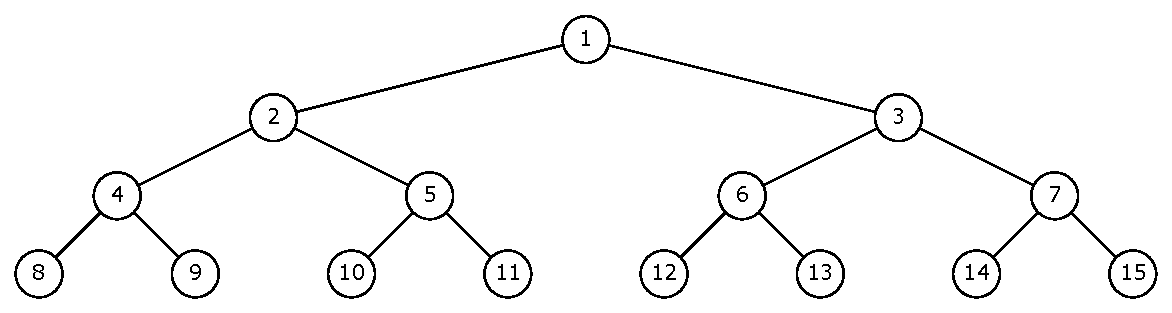
\includegraphics[width=\linewidth]{report/level_order.pdf}
    \caption{A perfect tree of height 3, where the numbers correspond to the order in which nodes are visited in a level order traversal}
\end{figure}

\begin{defn}[Preorder Traversal]
    In a preorder traversal, the root is visited first. Then, the procedure is called recursively on the left subtree, and then recursively on the right subtree. A preorder traversal is a form of depth-first search.
\end{defn}

\begin{figure}[H]
    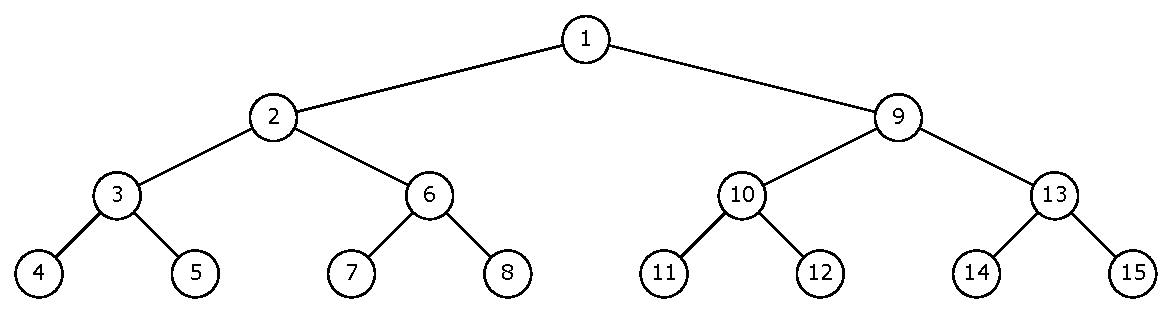
\includegraphics[width=\linewidth]{report/preorder.pdf}
    \caption{A preorder traversal in a perfect tree of height 3}
\end{figure}

\iffalse
\section{Reingold-Tillford (1981)}
One classic algorithm used to layout binary trees is described by Reingold and Tillford. 

\begin{figure}[H]
    \includegraphics[width=\linewidth]{"report/tree_2".pdf}
    \caption{A complete binary tree}
\end{figure}

\begin{figure}[H]
    \centering
    \begin{subfigure}{.5\textwidth}
        \centering
        \includegraphics[width=2in]{"report/figure2".pdf}
        \caption{An example of a tree generated by RT 81}
        \label{fig:fig2}
    \end{subfigure}%
    \begin{subfigure}{.5\textwidth}
        \centering
        \includegraphics[width=2in]{"report/figure4".pdf}
        \caption{Unlike other algorithms, RT 81 draws a tree and its mirror symetrically}
    \end{subfigure}%
    
    \caption{A reproduction of some figures from RT's original paper}
\end{figure}

\begin{figure}[H]
    \includegraphics[width=\linewidth]{"report/figure2_contours".pdf}
    \caption{The left contour and right contour of the same tree}
\end{figure}

\subsection{Algorithm Description}
\subsubsection{Informal Description}
First, we calculate the displacements of the nodes relative to each other.

\begin{enumerate}
    \item Base Case: Trivial
    \item Apply this algorithm to subtrees via a postorder traversal
    \item For each subtree, merge them horizontally such that they are two units apart horizontally
\end{enumerate}

\subsubsection{Formal Description}
\paragraph{Node Type}
To implement the tree in a programming language, we will need to creature a structure that represents each node in the tree.
\begin{labeling}{alligator}
    \item [left] Pointer to left subtree
    \item [right] Pointer to right subtree
    \item [offset] Offset relative to parent
\end{labeling}

By using offsets relative to a node's parent, as opposed to absolute offsets, we avoid having to reposition all of the nodes in a subtree when the root of that subtree gets moved.

\begin{algorithm}
    \caption{Reingold and Tilford's Algorithm}\label{euclid}
    \begin{algorithmic}[1]
        \Statex Constants:
        \Statex $minsep$: The smallest distance any two subtrees can be separated by [units]
        \Statex
        \Statex Input:
        %\hspace{\parindent}
        \Statex $t$: A binary tree
        \Statex
        
        % Begin Describing Algorithm   
        \Procedure{setup}{$t$}
        \State $cursep = minsep$ \Comment{Used to keep track of how far apart subtrees are}        
        \State setup(t$\rightarrow$left) \Comment{Post-order traversal on tree}
        \State setup(t$\rightarrow$right)
        
        % Begin Push
        \State $left \gets t\rightarrow left$
        \State $right \gets t\rightarrow right$
        \While{left is not NULL right is not NULL} \Comment{We only have to traverse as deep as the shortest subtree }
        \If{$cursep < minsep$} \Comment{Trees too close, so push them apart}
        \State $left\_dist \gets left\_dist + (minsep - cursep)/2$        
        \State $right\_dist \gets right\_dist + (minsep - cursep)/2$
        \State $cursep = minsep$
        \EndIf
        
        % Left->right
        \If{$left \rightarrow right$ not null} \Comment{Traverse left subtree}
        \State $left \gets left \rightarrow right$
        \State $cursep \gets cursep - left.offset$
        
        % Left->left
        \Else
        \State $left \gets left \rightarrow right$
        \State $cursep \gets cursep - left.offset$
        \EndIf
        
        % Right->left
        \If{$right \rightarrow left$ not null} \Comment{Traverse right subtree}
        \State $right \gets right \rightarrow left$
        \State $cursep \gets cursep - right.offset$
        \EndIf
        
        % Right->right
        \If{$left \rightarrow right$ not null}
        \State $right \gets right \rightarrow right$
        \State $cursep \gets cursep - right.offset$
        \EndIf
        
        \EndWhile\label{euclidendwhile}
        
        % Threading
        \If{$left$} \Comment{The left subtree was taller}
        \State Insert a thread from the right-most item of the right subtree to $right$
        \EndIf
        
        \If{$right$} \Comment{The right subtree was taller}
        \State Insert a thread from the left-most item of the left subtree to $right$
        \EndIf
        
        \EndProcedure
    \end{algorithmic}
\end{algorithm}

\subsubsection{Threading}
For every node in a given tree, the algorithm traverses through the left contour of the right subtree, and the right contour of the left subtree. In this traversal, the goal is to find the appropriate number units to separate the trees by. However, for any given node, its right contour may not be contained entirely within the same subtree. Hence, we require "threads", or connections between nodes in different subtrees in order to follow a tree's contour. Per the visualization below, we may think of threads as temporary edges.

\begin{figure}[H]
    \centering
    \includegraphics[width=4in]{"report/figure2_threads".pdf}
    \caption{Threads (dashed) created by the algorithm while traversing the tree in Figure \ref{fig:fig2} }
\end{figure}

\subsection{Algorithm Trace for Complete Binary Trees}
The figures below show the displacements set by the algorithm for each node. From these figures, we can see how the algorithm achieves symmetry between subtrees.

\begin{figure}[H]
    \centering
    \includegraphics[width=4in]{"report/figure2_labels".pdf}
    \caption{Algorithm trace for example tree}
\end{figure}

\begin{figure}[H]   
    \includegraphics{"report/binary_tree_1".pdf}
    \linebreak
    
    \includegraphics{"report/binary_tree_2".pdf}
    \linebreak
    
    \includegraphics{"report/binary_tree_3".pdf}
    \linebreak
    
    \includegraphics[width=\linewidth]{"report/binary_tree_4".pdf}
    \linebreak
    
    \includegraphics[width=\linewidth]{"report/binary_tree_5".pdf}
    \linebreak
    
    \caption{Algorithm trace for complete binary trees of heights 2 through 6}
\end{figure}
\fi

\section{Tree Drawing as a Linear Program -- Supowit and Reingold (1983)}
\subsection{The Problem of Narrow Trees}
Unfortunately, as shown earlier (note to self: show earlier), locally minimizing the width of every subtree does not achieve the goal of a minimum width drawing. Sometimes in order to draw a tree as narrow as possible, some subtrees have to be drawn non-optimally.

\subsection{Aesthetic Trees}

In the algorithm below, the problem of drawing a tree is formulated as a linear program.\cite{supowit1983complexity} Although linear time algorithms exist for drawing trees, they do not necessarily produce ``nice'' drawings. In Supowit and Reingold's paper, the problem of drawing a tree can be described as finding the narrowest possible drawing such that it matches several aesthetics:
\begin{enumerate}
    \item \textbf{Layering} All nodes at the same level, i.e. the number of edges between a node and the root, share the same y-coordinate
    \item \textbf{Child Positioning} Each left child is placed strictly to the left of its parent, and each right child is placed strictly to the right of its parent
    \item \textbf{Separation} For any two nodes at the same level, they must be placed at least 2 units apart.
    \item \textbf{Centering} If a parent has two children, then it must be centered over them
    \item \textbf{Planarity} No two tree edges may be drawn such that they intersect, unless they same a common vertex
    \item \textbf{Isomorphic Trees Drawn Similarly} If two subtrees are isomorphic, they must be drawn identically (minus a translation)
\end{enumerate}

As Theorem \ref{tree_lp_planar} shows, enforcing aesthetics 1, 2 and 3 are sufficient to guarantee 5.

\bigskip

By formulating the problem using linear programming, the time complexity of tree drawing can be reduced to polynomial time.\cite{supowit1983complexity}

\subsection{Formal Description}
First, define $f$ to be a mapping from a tree's vertex set to $\mathbb{R}^2$. Trivially, we can satisfy Aesthetic 1 by defining $f_y(n) = -i$ where $i$ is the level of node $n$. Then, we use a linear program to determine the value of $f_x(n)$. We will introduce two auxiliary variables $x_{max}$ and $x_{min}$ which give the left and right bounds for the x-coordinates of our drawing respectively. Hence, our goal of creating the narrowest possible drawing may be expressed as 
\[
\min{x_{max} - x_{min}}
\]

subject to:

\[
\begin{aligned}
    &f_x(n) \geq x_{min} \\
    &f_x(n) \leq x_{max} \\
    &f_x(n) - f_x( \leftc{n} ) \geq 1 &\text{For all $n$ with a left child (Aesthetic 2)} \\
    &f_x( \rightc{n} ) - f_x(n) \geq 1 &\text{For all $n$ with a right child (Aesthetic 2)} \\
    &f_x(n) - f_x(m) \geq 2 &\text{$n$ is the level-order successor of $m$ (Aesthetic 3)} \\
    &\frac{ f_x(\leftc{n}) + f_x(\rightc{n}) }{2} = f_x(n)
         &\text{For all $n$ with two children (Aesthetic 4)} \\
\end{aligned}
\]

Lastly, to implement aesthetic 6, for every node in the tree, we determine its rank and the number of in the subtree rooted at that node. Hence, we can partition every node in the tree into an equivalence classes where we say--for any nodes $m, n$--$m$ is equivalent to $n$ if they have the same size and rank. Then, for each equivalence class with more than one member, we require the constraints. Let $\{ n_1, n_2, ..., n_k \}$ be the members of some equivalence class. Then, we require the constraints

\begin{equation}
    f_x( \rightc{n_i} ) - f_x(n_i) = f_x( \rightc{n_{i + 1}} ) - f_x( n_{i + 1} )
\end{equation}

\begin{equation}
    f_x( n_i ) - f_x( \leftc{n_i} ) = f_x( n_{i + 1} ) - f_x( \leftc{n_{i+1}} )
\end{equation}

Because, corresponding subtrees in isomorphic trees are also isomorphic, the equations above are sufficient to satisfy Aesthetic 6. (Reword this)

\begin{figure}[H]
    \centering
    \includegraphics[width=\linewidth]{"report/full_tree".pdf}
    \caption{A drawing of a perfect tree of height 4}
\end{figure}

\begin{theorem}[Planarity]
    \label{tree_lp_planar}
    Let $T$ be any binary tree drawn by this algorithm. Then, aesthetics 1, 2, and 3 imply aesthetic 5.
    
    \begin{proof}
        First, if every node $n$ on some level $i$ is drawn according to the rule $f_y(n) = -i$, then ensuring planarity simply means ensuring nodes on the same level do not cross. We will show via induction on the height of the tree that given aesthetic 1, aesthetics 2 and 3 then imply 5.
        
        \bigskip
        
        \paragraph{Base Case} Trivially, this algorithm gives a planar drawing for a tree of height 0.
        
        % Cheeky
        \begin{figure}[H]
            \centering
            \includegraphics[height=0.5in]{"report/perfect_tree_0".pdf}
            \caption{The full tree of height 0 as drawn by this algorithm}
        \end{figure}
        
        \paragraph{Inductive Hypothesis} Assuming that the previous $i - 1$ levels of the tree are drawn in a planar fashion, we will show that for any node in the $i^{th}$ level, the edge between it and its parent does not intersect any other edges.
        
        \bigskip
        
        First, suppose for a contradiction that there is some edge crossing. This implies one of three cases. It may be because some node's right subtree crosses some other node's left subtree or vice-versa.
        
        \begin{figure}[H]
            \centering
            \includegraphics[height=0.5in]{"report/planarity_cx1".pdf}
            \caption{A right subtree crossing with a left subtree}
        \end{figure}
        
        However, this implies a violation of aesthetic 3 as the left subtree of the right parent should be drawn to the right of the right subtree of the left parent. Moreover, there may be a crossing since some node's left subtree crosses some other node's left subtree. However, this either implies the subtrees are drawn directly on top of each other (a violation of aesthetic 3), or that a ``left'' subtree is drawn to the right of its parent, which is a violation of aesthetic 2.
        
        \begin{figure}[H]
            \centering
            \includegraphics[height=0.5in]{"report/planarity_cx2".pdf}
            \caption{Here, two ``left'' subtrees (colored in red) cross each other}
        \end{figure}
        
        Lastly, it may be that some node's right subtree crosses some other node's right subtree. But, with logic similar to the case above, this either implies a violation of aesthetic 2 or 3.
        
        \begin{figure}[H]
            \centering
            \includegraphics[height=0.5in]{"report/planarity_cx3".pdf}
            \caption{Here, two ``right'' subtrees (colored in blue) cross each other}
        \end{figure}
    \end{proof}
\end{theorem}

\begin{theorem}[Number of Constraints]
    The number of constraints is $O(n)$.
    
    \begin{proof}
        Let $T$ be a binary tree with $n$ nodes. First, the requirements $x_{min} \leq f_x(n)$ and $f_x(n) \leq x_{max}$ contribute $2n$ constraints.
        
        \paragraph{Aesthetic 2} For any tree, every node except the root is either a left or right son. Hence, there aesthetic 2 contributes $n - 1$ constraints.
        
        \paragraph{Aesthetic 3} For every level, this aesthetic requires a constraint for every adjacent pair of nodes. There are less pairs than nodes, so this quantity is less than $n$.
        
        \paragraph{Aesthetic 4} For any tree, there are less parents than total nodes, so this aesthetic requires no more than $n$ constraints.
        
        \paragraph{Aesthetic 6} There less than $\frac{n}{2}$ equivalence classes (excluding the equivalence class of leaves) with more than one member, so this constraint contributes no more than $\frac{n}{2}$ constraints.
        
        \bigskip
        
        Hence, we can see that there are at most $6n$ aesthetic constraints, so the number of constraints is $O(n)$ as required.
    \end{proof}
\end{theorem}

\begin{theorem}[Number of Constraints of a Perfect Tree]
    For a perfect tree of height $h$, this algorithm requires
    \[ \left( 4\sum_{i=0}^h 2^i \right) - 2h - 2^{h+1} - 3 \]
     constraints.
    
    \begin{proof}
        To begin, in a perfect binary tree, the number of nodes at every level doubles. Hence, in a perfect tree of height $h$, there are 
        $\sum_{i=0}^h 2^i$ nodes. Because all of the constraints are somehow related to this number, we'll denote this quantity as $t$.
        
        \paragraph{Width Constraints} For every node in the tree, a pair of constraints is required for the auxiliary variables $x_{max}$ and $x_{min}$. Hence, there are $2t$ of these constraints.
        
        \paragraph{Aesthetic 2} Every node in the tree except the root is either a left or a right son, so this aesthetic requires $t - 1$ constraints.
        
        \paragraph{Aesthetic 3} For each level in this tree with $k > 1$ nodes (i.e. every level except the one containing the root), this constraints necessitates $k - 1$ constraints. Hence, we need 
        \[
            (2^1 - 1) + (2^2 - 1) + ... + (2^h - 1) = t - (h + 1)
        \]
        
        constraints to satisfy this aesthetic.
        
        \paragraph{Aesthetic 4} Every node in a perfect tree except for those at the last level have two children, hence we need
        \[
            2^0 + 2^1 + ... + 2^{h-1} = t - 2^h
        \]
        constraints to satisfy this aesthetic.
        
        \paragraph{Aesthetic 6} For any given level, every node in that level is isomorphic to other nodes in that level. In other words, each level of the perfect tree except for the root forms an equivalence class. Recall, for the purpose of aesthetic 6 we ignore every leaf node. Hence, the equivalence classes are composed of every node in the tree except for the root and last level. For each level, we add a constraint for every pair of adjacent nodes. Hence, we need
        \[
            (2^1 - 1) + ... + (2^{h - 1} - 1) = t - (2^h + h + 1)
        \]
        constraints for this aesthetic.
        
        \bigskip
        
        Adding this all up, we get $4t - 2h - 2^{h+1} - 3$ constraints.
    \end{proof}
\end{theorem}

\subsection{Implementation}
In this paper, this algorithm was implemented as a C++ program based around the GNU Linear Programming Kit (GLPK)--an open-source linear optimizer based on the simplex method.\cite{glpk} Each node (in the C++ implementation--struct TreeNode) was represented as a data structure as follows:

\begin{labeling}{alligator}
    \item [left]  Pointer to left child
    \item [right] Pointer to right child
    \item [id]    Corresponding column index of constraint matrix
    \item [data]  Self-explanatory
\end{labeling}

Then, aesthetics 1-5 could be computed using $2n$ iterations. First, an iterative level-order traversal was used to simultaneously assign IDs to each node, determine the number of left and right sons, and thus, determine the total number of rows and columns in the constraint matrix. By using an iterative method, our traversal took linear as opposed to quadratic time. During the level-order traversal, a hash table mapping each level of the tree to an array of node pointers was populated.
\footnote{Implemented in C++ as \lstinline{std::unordered_map<int, TreeNode*>}}
Then, a final iteration over this auxiliary data structure was used to calculate the aesthetics. (Write about how paper uses a different method).

\bigskip

It should be noted that regardless of method used, computing the required aesthetics requires at least two iterations, where the first iteration is used to assign column indicies to nodes. If the first iteration is a level-order traversal, then we cannot calculate any constraints related to a node's children until a second traversal--since the children do not have column indices assigned. On the other hand, if an initial preorder traversal is used, then we will still need a second iteration to calculate the third aesthetic since we are not aware of all of the nodes on one level during a preorder traversal.

\bigskip

Finally, in order to populate the auxiliary data structure, for every node, we also had to keep track of which level it was on. To accomplish this during an iterative level-order traversal, each node pointer was paired with its current level (e.g. (\lstinline{std::pair<int, TreeNode*>})). As shown in the pseudocode below, each pointer's associated level can be determined when we examine its parent.

\begin{algorithm}[H]
    \caption{Tree Layout -- Column Index Assignment}
    \label{tree_lp_initial}
    \begin{algorithmic}[1]
        % Begin Describing Algorithm
        \Procedure{assign\_ids}{$t$}
        \State Create a queue $children$ initially populated with the pair $(0, root)$ where 0 is the level of root
        \State $num\_nodes \gets 0$ \Comment{Information for constraint matrix}
        \State $left\_sons \gets 0$
        \State $right\_sons \gets 0$
        \State $current\_id \gets 0$ \Comment{Corresponding column of constraint matrix}
        \While{$children$ is not empty} \Comment{Level-order traversal}
        \State Pop the first element from $children$ and assign it to $current$
        \State $current\_level \gets current.first$
            \Comment{$current =$ (level (integer), node pointer)}
        \State $current\_node \gets current.second$
        \State $current\_node\rightarrow id \gets current\_id$
            % Left child
            \If{$current\_node\rightarrow left$ is not null}
            \State $children \gets (current\_level + 1, root\rightarrow left)$ \Comment{Determine level of child}
            \State $left\_sons \gets left\_sons + 1$ \Comment{Keep count of left sons (aesthetic 2)}
            \EndIf
            % Right child
            \If{$current\_node\rightarrow right$ is not null}
            \State $children \gets (current\_level + 1, root\rightarrow right)$ \Comment{Determine level of child}
            \State $right\_sons \gets right\_sons + 1$ \Comment{Keep count of right sons (aesthetic 2)}
            \EndIf
        \State $levels[current\_level].push\_back(current\_node)$
            \Comment{Update mapping of levels to their nodes}
        \State $current\_id \gets current\_id + 1$
        \EndWhile
        \EndProcedure
    \end{algorithmic}
\end{algorithm}

After the column indices have been assigned, we can then easily calculate aesthetics 1 through 5 using the mapping $levels$ from algorithm \ref{tree_lp_initial}.

\begin{algorithm}[H]
    \caption{Tree Layout -- Calculating Aesthetics 1-5}
    \begin{algorithmic}[1]
        % Begin Describing Algorithm
        \Procedure{calculate\_constraints}{$levels$}
        \For{level $l = 0, ..., h$}
            \For{node $i = 0, ..., m$} \Comment{Iterate over nodes at level $l$, where $m$ is the number of nodes at level $l$}
            \State Let $current\_node$ refer to $levels[l][i]$ (the $i^{th}$ node at level $l$)
            \State Add constraint $current\_node \leq x_{max}$ \Comment{Add width constraints}
            \State Add constraint $current\_node \geq x_{min}$
            \If{$current\_node \rightarrow left$ is not null}
                \State Add second constraint
            \EndIf
            \If{$current\_node \rightarrow right$ is not null}
                \State Add second constraint
            \EndIf
            \If{$current\_node \rightarrow left$ and $current\_node \rightarrow right$ are not null}
                \State (Add parent centered constraint)
            \EndIf
            \If{$i < n$}
                \State Add separation constraint
            \EndIf
            \EndFor
        \EndFor
        \EndProcedure
    \end{algorithmic}
\end{algorithm}

Thus, calculating the first five aesthetics can be done in linear time by iterating over each node just twice.

\subsection{Aesthetic 6 -- Drawing Isomorphic Trees Identically}
As mentioned by the paper's authors, there is some debate about whether or not this should be considered an aesthetic. However, sometimes visualizations are used to find recurring patterns, and enforcing this aesthetic allows humans to more effectively use their pattern recognition abilities. In Figure \ref{fig:aes6_on_off}, the same tree is drawn twice by this algorithm, where aesthetic 6 is relaxed in the first drawing.

\begin{figure}[H]
    \label{fig:aes6_on_off}
    \begin{subfigure}{\linewidth}
        \centering
        \includegraphics[width=\linewidth]{"report/no_aes6_20".pdf}
        \caption{An incomplete tree of height 20 as drawn by this algorithm satisfying aesthetics 1-5}
    \end{subfigure}
    
    \begin{subfigure}{\linewidth}
    \centering
    \includegraphics[width=\linewidth]{"report/aes6_20".pdf}
    \caption{An isomorphic tree as drawn by this algorithm satisfying aesthetics 1-6}
    \end{subfigure}
    \caption{Two drawings of isomorphic trees differing only in the application of aesthetic 6}
\end{figure}

\subsubsection{Rank of a Tree}
In order to efficiently draw isomorphic trees identically, we define a function $rank()$ which assigns a unique integer to every binary tree. We must be careful and note that this number is unique among trees of the same size, as trees of different size may be assigned the same number. Hence, we can say two subtrees are isomorphic if they have the same size and rank.

\bigskip

Knott showed that this function is one-to-one (among trees of the same size) and that the numbering it generated corresponded to an ordering among trees.~\cite{Knott:1977:NSB:359423.359434} For even $n$, there are $B_n = \frac{ \binom{2n}{n} }{ n + 1 }$ different binary trees, so we can say $rank(t)$ is a mapping from the trees $t$ of size $n$ to the integers $1, 2, ..., B_n$.
\begin{algorithm}[H]
    \caption{Tree Layout -- Calculating the Rank of Each Node}
    \begin{algorithmic}[1]
        % Begin Describing Algorithm
        \Procedure{rank}{$t$, $cache$}        
        \If{$t$ is null}
            \State $rank \gets 1$
        \Else
            \State $rank \gets B_n(r(t)) \times rank(l(t) - 1) + rank(r(t)) + \sum G_{j,n}$
        \EndIf
        \State $cache[size(t)][rank].push\_back(tree)$
        \State \Return $rank$
        \EndProcedure
    \end{algorithmic}
\end{algorithm}

In the algorithm above, the $rank()$ of a tree is computed recursively, moving from the bottom up. Hence, calling $rank()$ on the root node has the effect of computing the $rank()$ of every node in the tree. As a result, it behooves us to cache the calls of $rank()$. Specifically, in this implementation, the cache is a mapping of a subtree's size and rank to an array of trees of similar size and rank (i.e. isomorphic subtrees).\footnote{In C++, the author choose to implement the cache as \\ \lstinline{std::unordered_map<int, std::unordered_map<int, std::vector<TreeNode*>>>})} Hence, implementing the sixth aesthetic is simply a matter of iterating over the arrays of this cache.

\begin{sidewaysfigure}
    \centering
    \includegraphics[width=\linewidth]{"report/bst_large".pdf}
    \caption{A binary search tree with 50 items}
\end{sidewaysfigure}

\pagebreak

\chapter{Force Directed Algorithms}
\section{Introduction}
Force directed algorithms attempt to draw graphs by relating them to some physical analogy. For example, we may view vertices as steel balls and the edges between them as springs. One of the earlier force directed algorithms, Tutte's Barycenter Algorithm, attempts to place a graph's nodes along it's "center of mass."

\subsection{Notation}
Although there are plenty of force-directed algorithms, they all have the final result of mapping the vertices of a graph to $\mathbb{R}^2$. Hence, we saw that each vertex $v$ in a graph gets mapped to some point $p_v = (x_v, y_v)$. 

\section{Eades' Spring System}
In this algorithm, edges are modeled as springs while vertices are viewed as electrical forces which repel each other.~\cite{eades1984heuristic} Formally, the force on each vertex $v$ is 
\[
    F(v) = \sum_{(u, v) \in E} f_{uv} + \sum_{(u, v) \in V \times V} g_{uv}
\]

If we use Hooke's law springs and electrical forces which follow an inverse square law, we can write this as

\[
    \sum_{(u, v) \in E} k_{uv}^{(1)} ( d(p_u, p_v) - l_{uv} ) \frac{x_v - x_u}{d(p_u, p_v)} +
    \sum_{(u, v) \in V \times V} \frac{k_{uv}^{(2)}}{( d(p_u, p_v) )^2 }  \frac{x_v - x_u}{d(p_u, p_v)}
\]

\subsection{Algorithm}
A very simple algorithm for finding the system's equilibrium is to move each vertex in the direction of the force in a small proportion to the magnitude of the force. An example of this algorithm at work drawing $K_8$ is shown below

\begin{figure}[H]
    \centering
    \includegraphics[width=\linewidth]{"report/k8_trace".pdf}
    \caption{The complete graph $K_8$}
\end{figure}

\begin{figure}[H]
    \centering
    \includegraphics[width=\linewidth]{"report/tesseract".pdf}
    \caption{The tesseract $Q_4$}
\end{figure}

\subsection{Sensitivity to Initial Positions}
As notice, this algorithm is best described as a "heuristic."   

\begin{figure}[H]
    \begin{subfigure}{.5\linewidth}
    \centering
    \includegraphics[width=\linewidth]{"report/cube_random".pdf}
    \end{subfigure}
    \begin{subfigure}{.5\linewidth}
    \centering
    \includegraphics[width=\linewidth]{"report/cube".pdf}
    \end{subfigure}
    \caption{Two drawings of the cube $Q_3$}
\end{figure}

\section{Tutte's Barycenter Method}
An early force directed drawing method was Tutte's Barycenter Method.~\cite{tutte1963draw} In this method, the force on every vertex $v$ is given by 

\begin{equation}\label{eq:barycenter}
F(v) = \sum_{(u, v) \in E} (p_u - p_v)
\end{equation}

Hence, splitting (\ref{eq:barycenter}) across the x and y dimensions we get
\begin{equation}\label{eq:barycenter_split}
    \begin{aligned}
    \sum_{(u, v) \in E} (x_u - x_v) &= 0 \\
    \sum_{(u, v) \in E} (y_u - y_v) &= 0 \\
    \end{aligned}
\end{equation}

\subsection{Fixed Vertices}
However, notice the system in (\ref{eq:barycenter_split}) has the trivial solution $(x, y) = (0, 0)$ for all vertices, which gives a very poor drawing! Hence, we take $n \geq 3$ vertices such that they form a convex polygon, and fix them. \\

In this paper's implementation of the algorithm, the fixed vertices are positioned as $n$ equally spaced points along a circle of radius equal to half the width of the final image, centered at the origin.

\subsection{Linear Model}
Suppose for some free vertex $v$, we denote the set of fixed neighbors as $N_0$, and the set of free neighbors as $N_1$. Then, we may rewrite the above equations as

\begin{equation}\label{eqn:barycenter_linear}
    \begin{aligned}
        \deg{(v)}x_v - \sum_{u \in N_1(v)} x_u &= \sum_{w \in N_0(v)} x^*_w \\
        \deg{(v)}y_v - \sum_{u \in N_1(v)} y_u &= \sum_{w \in N_0(v)} y^*_w
    \end{aligned}
\end{equation}

Hence, for every free vertex, there is a pair of equations (one for x, and one for y). These equations are linear, and after labeling the free vertices $v_1, ..., v_n$, we may rewrite them as the matrix multiplications described in (5) and (6) below. Notice the $M$ is an $n \times n$ diagonally dominant matrix. The first fact can be observed by inspecting \ref{eqn:barycenter_linear}, and the second occurs because the diagonal consists of vertex degrees, while the other entries $M_{ij}$ are either -1's (if $x_i$ and $x_j$ are neighbors) or 0's if they aren't. Formally, this matrix $M$ is known as the \textbf{Laplacian} of the graph.

\begin{equation}\label{eqn:barycenter_matrix}
    M_{ij} = \begin{cases}
    \deg(v) &{\text{if $i = j$}} \\
    -1      &{\text{if adjacent}} \\
    0       &{\text{otherwise}} \\
    \end{cases}
    \equiv
    \begin{bmatrix}
    \deg(v) &        &        & * \\
            & \ddots &        & \\
            &        & \ddots & \\
    *       &        &        & \deg(v) \\
    \end{bmatrix}
\end{equation}

We may find the x coordinates of the free vertices by solving

\begin{equation}\label{eqn:barycenter_matrix_x}
    M \begin{pmatrix}
        x_1 \\ \vdots \\ x_n \\
    \end{pmatrix} =
    \begin{pmatrix}
        \sum_{w \in N_0(x_1)} x^*_w \\
        \vdots \\
        \sum_{w \in N_0(x_n)} x^*_w \\
    \end{pmatrix}
\end{equation}

and the y coordinates by solving

\begin{equation}\label{eqn:barycenter_matrix_y}
    M \begin{pmatrix}
       y_1 \\ \vdots \\ y_n \\
    \end{pmatrix} =
    \begin{pmatrix}
        \sum_{w \in N_0(y_1)} y^*_w \\
        \vdots \\
        \sum_{w \in N_0(y_n)} y^*_w \\
    \end{pmatrix}
\end{equation}

\subsection{Example: Hypercube}
A simple example for which Tutte's method gives aesthetically pleasing results is the hypercube.

\begin{figure}[H]
    \centering
    \includegraphics[width=0.5\linewidth]{"report/prism_4".pdf}
    \caption{The hypercube $Q_3$}
    \label{fig:hypercube}
\end{figure}

In Figure \ref{fig:hypercube} the hypercube is placed in 500 x 500 pixel grid. The grid is governed by a simple Cartesian coordinate system, where the top left and bottom right corners have coordinates $(-250, 0)$ and $(250, 250)$ respectively. Four vertices are fixed and laid out into a circle of radius 250 centered at the origin. Hence, the bulk of the work performed algorithm is done in placing the center four free vertices. Labeling the free vertices as $x_1, x_2, x_3, x_4$, we may represent the task of laying out the free vertices with this matrix

\[
\begin{bmatrix}
    3 & -1 & 0 & -1 \\
    -1 & 3 & -1 & 0 \\
    0 & -1 & 3 & -1 \\
    -1 & 0 & -1 & 3 \\
\end{bmatrix}
\begin{bmatrix} x_1 \\ x_2 \\ x_3 \\ x_4 \end{bmatrix} =
\begin{bmatrix} 0 \\ 250 \\ 0 \\ -250 \end{bmatrix}
\]

The solution to this matrix is given by $x_1 = x_3 = 0, x_2 = \frac{250}{3}, x_4 = -\frac{250}{3}$.

\subsection{Algorithms}
\subsubsection{Newton-Raphson Iteration}
The below Newton-Raphson Iteration is easy to code and is reasonably fast. However, it is not as fast as solving Algorithm \ref{barycenter_la} below with a linear algebra package. The idea behind the algorithm is that we simply keep iterating until the $x, y$ values of each vertex converges. However, this implies we need to define convergence in a way dumb enough for a computer to understand.

\begin{defn}[Convergence]
    Let $p_{i - 1}, p$ be the placement of some vertex $v$ during the $i - 1$ and $i^{th}$ iteration of the Newton-Raphson Iteration. We say that $p$ has converged if $\abs{p - p_{i - 1}} < \epsilon$. (In practice, we can define $\epsilon$ to be a very small positive number like $0.01$).
\end{defn}

\begin{algorithm}[H]
    \caption{Barycenter Layout (Newton-Raphson)}
    \begin{algorithmic}[1]
        % Begin Describing Algorithm
        \Procedure{barycenter}{$t$}
        \State Place each fixed vertex $u \in V_0$ at a vertex of $P$ and each free vertex at the origin.
        \State $converge \gets false$
        \While{$!converge$}
            \State $converge \gets true$
            \For{each free vertex $v$}
                \[
                \begin{aligned}
                x_v &= \frac{1}{\deg{v}} \sum_{(u, v) \in E} x_u \\
                y_v &= \frac{1}{\deg{v}} \sum_{(u, v) \in E} y_u \\
                \end{aligned}
                \]
                
                \State \text{// If this does not execute at any point in the for loop, then while loop exists}
                \If{$p$ did not converge}
                    \State $converge \gets false$
                \EndIf
            \EndFor
        \EndWhile
        \EndProcedure
    \end{algorithmic}
\end{algorithm}

\subsubsection{Linear System}
Of course, with a computer linear algebra package (such as Eigen for C++),~\cite{eigen} one can also solve the corresponding linear system directly. In practice, this tends to be significantly faster than the previous algorithm.

\begin{algorithm}[H]
    \caption{Barycenter Layout (Linear Algebra)}\label{barycenter_la}
    \begin{algorithmic}[1]       
        % Begin Describing Algorithm   
        \Procedure{barycenter}{$t$}
        \State Layout $n$ fixed vertices in a convex polygon
        \State Construct a matrix $M$ as described by (\ref{eqn:barycenter_matrix})
        \State Construct a vector of $x$-coordinates for free vertices and another for fixed vertices. Along with $M$, use these to solve (\ref{eqn:barycenter_matrix_x})
        \State Construct a vector of $y$-coordinates for free vertices and another for fixed vertices. Along with $M$, use these to solve (\ref{eqn:barycenter_matrix_y})
        \EndProcedure
    \end{algorithmic}
\end{algorithm}

\subsection{Case Study: Prism Graph}
The prism graph $\Pi_{n}$ is a 3-connected graph constructed by taking the vertices and edges of an $n$-prism. From the perspective of this drawing algorithm, it allows us to investigate the symmetry and resolution properties. In this paper, and the proofs below, $\Pi_{n}$ will be drawn by using $n$ fixed vertices (equally spaced on the perimeter of a circle).

\begin{figure}[H]
    \centering
    
    \begin{subfigure}{.3\textwidth}
        \includegraphics[width=\linewidth]{"report/prism_4".pdf}
    \end{subfigure}
    \begin{subfigure}{.3\textwidth}
        \includegraphics[width=\linewidth]{"report/prism_5".pdf}
    \end{subfigure}
    \begin{subfigure}{.3\textwidth}
        \includegraphics[width=\linewidth]{"report/prism_6".pdf}
    \end{subfigure}

    \begin{subfigure}{.3\textwidth}
        \includegraphics[width=\linewidth]{"report/prism_7".pdf}
    \end{subfigure}
    \begin{subfigure}{.3\textwidth}
        \includegraphics[width=\linewidth]{"report/prism_8".pdf}
    \end{subfigure}
    \begin{subfigure}{.3\textwidth}
        \includegraphics[width=\linewidth]{"report/prism_9".pdf}
    \end{subfigure}
    \caption{$\Pi_4$ through $\Pi_{9}$ as drawn by Tutte's algorithm. Notice that $\Pi_4$ is isomorphic to the hypercube $Q_3$}
\end{figure}

\subsubsection{Symmetry}
Under certain conditions, the barycenter method produces drawings which preserve symmetry.

\begin{theorem}[Eigenvectors of the Prism Graph]
    Consider the linear system governing the coordinates of the free vertices of the prism graph $\Pi_n$. Now, take its corresponding matrix $M$ and starting at $(1, 0)$, place $n$ points equally along the perimeter of the unit circle. If we create vectors $x = (x_1, ..., x_n), y = (y_1, ..., y_n)$, where $x_i$ is the x-coordinate of the $i^{th}$ unit circle point (and similarly for $y$), then $x, y$ are eigenvectors for $M$ with corresponding eigenvalues
    $\lambda_x = \lambda_y = 3 - 2 \cos{\frac{2\pi}{n}}$.
    
    \begin{proof}
        First, let us prove that this is true for $x$. Notice by the distributivity of linear maps that $Mx = (3I + N)x = 3Ix + Nx$, where $N$ is a matrix composed of all of the $-1's$ in $M$ (and is zero everywhere else). Hence, $N\vec{x}$ is of the form
        \[
        \begin{bmatrix}
        0  & -1     & 0      & \dots   & 0      & -1 \\
        -1 & \ddots & \ddots & \ddots  & \ddots & 0 \\
        0  & \ddots & \ddots & \ddots  & \ddots & 0 \\
        0  & \ddots & \ddots & \ddots  & \ddots & 0 \\
        0  & \ddots & \ddots & \ddots  & \ddots & -1 \\
        -1 & 0      & \dots  & 0       & -1     & 0 \\
        \end{bmatrix}
        \begin{bmatrix}
            \cos{0} \\ 
            \cos{\frac{2 \pi}{n}} \\
            \vdots \\
            \cos{\frac{2 \pi(n-2)}{n}} \\
            \cos{\frac{2 \pi(n-1)}{n}}
        \end{bmatrix}
        \]
        
        Clearly, any vector is an eigenvector of the identity map, so we just have to show that $x$ is an eigenvector of $N$. By the above matrix, showing that $Nx = \lambda_0 x$ is equivalent to showing that the following holds for some $\lambda_0 \in \mathbb{R}$.
        
        \[\begin{cases}
        -\cos{\frac{2 \pi}{n}} - \cos{\frac{2\pi(n-1)}{n}} = \lambda_0 \cos{0} &\text{Equation for the first row} \\
        -\cos{\frac{2 \pi (i - 2)}{n}} - \cos{\frac{2 \pi i}{n}} = \lambda_0 \cos{\frac{2\pi(i-1)}{n}}
        &\text{Equation for the $i^{th}$ row} \\
        \end{cases}\]
        
        Now, the first equation implies that 
        \[\begin{aligned}
        \lambda_0
        &= -\left[
        \cos{\frac{2\pi}{n}} + \cos{\frac{2\pi n - 2\pi}{n}}   
        \right] \\
        &= -2\left[
        \cos{ \frac{
                2 \pi + 2\pi n - 2\pi    
            }{ 2n } }
        \cos{ \frac{
                2\pi - 2\pi n + 2\pi
            }{ 2n }
        } \right]
        &\text{Using sum-product identity} \\
        &= -2\left[
        \cos{ \frac{2 \pi n}{2n} } \cos{\frac{ 4\pi - 2\pi n }{2n} }
        \right] \\
        &= -2\left[
        \cos{ \pi } \cos{ \frac{ 2\pi}{n} - \pi }
        \right] \\
        &= 2\left[
        \cos{ \pi - \frac{ 2\pi}{n}} \right]
        &\text{cos is an even function} \\
        &= -2\cos{ - \frac{ 2\pi}{n} }
        = -2\cos{ \frac{ 2\pi}{n} }
        &\text{Supplementary angles}
        \end{aligned}\]
        
        implying that $\lambda_x = 3 - 2\cos{\frac{2\pi}{n}}$ as desired. Now, we just need to show the equation for the $i^{th}$ row holds. Notice that
        
        \[
        \begin{aligned}
        &-\left[\cos{\frac{2 \pi (i - 2)}{n}} + \cos{\frac{2 \pi i}{n}}\right] \\
        &= -2\left[
        \cos{ \frac{2\pi(i - 2) + 2\pi i}{2n} }
        \cos{ \frac{2\pi(i - 2) - 2\pi i}{2n} }
        \right]
        &\text{Sum-product identity} \\
        &= -2\left[
        \cos{ \frac{\pi i - 2\pi + \pi i}{n} }
        \cos{ \frac{\pi i - 2\pi - \pi i}{n} }
        \right] \\
        &= -2\left[
        \cos{ \frac{\pi i - 2\pi + \pi i}{n} }
        \cos{ \frac{2\pi}{n} }
        \right]
        &\cos{ \frac{-2\pi}{n} } = \cos{ \frac{2\pi}{n} } \\
        &= \lambda_0 \cos{ \frac{2\pi(i - 1)}{n} }
        \end{aligned}
        \]
        
        as desired.
        
        \bigskip
        
        Now, let us prove that this is true for $y$. The proof is very similar to the proof for $x$. Here, $N\vec{y}$ is of the form
        \[
        \begin{bmatrix}
        0  & -1     & 0      & \dots   & 0      & -1 \\
        -1 & \ddots & \ddots & \ddots  & \ddots & 0 \\
        0  & \ddots & \ddots & \ddots  & \ddots & 0 \\
        0  & \ddots & \ddots & \ddots  & \ddots & 0 \\
        0  & \ddots & \ddots & \ddots  & \ddots & -1 \\
        -1 & 0      & \dots  & 0       & -1     & 0 \\
        \end{bmatrix}
        \begin{bmatrix}
            \sin{0} \\ 
            \sin{\frac{2 \pi}{n}} \\
            \vdots \\
            \sin{\frac{2 \pi(n-2)}{n}} \\
            \sin{\frac{2 \pi(n-1)}{n}}
        \end{bmatrix}
        \]
        
        Equivalently, we want to show that the following holds for some $\lambda_1 \in \mathbb{R}$.
        
        \[\begin{cases}
        -\sin{\frac{2 \pi}{n}} - \sin{\frac{2\pi(n-1)}{n}} = \lambda_1 \sin{0} &\text{Equation for the first row} \\
        -\sin{0} - \sin{\frac{2\pi\cdot 2}{n}} = \lambda_1 \sin{\frac{2 \pi}{n}} &\text{Equation for the second row} \\
        -\sin{\frac{2 \pi (i - 2)}{n}} - \sin{\frac{2 \pi i}{n}} = \lambda_1 \sin{\frac{2\pi(i-1)}{n}}
        &\text{Equation for the $i^{th}$ row} \\
        \end{cases}\]
        
        Note that here, we'll fix $\lambda_1$ by using the equation for the 2nd row since in the first row, the right hand side is equal to 0. Now, the second equation implies that 
        \[\begin{aligned}
        \lambda_1 \sin{\frac{2\pi}{n}}
        &= -\left( \sin{0} + \sin{\frac{4\pi n}{n}} \right) \\
        &= -\sin{\frac{4\pi}{n}} \\
        &= -2\sin{\frac{2\pi}{n}}\cos{\frac{2\pi}{n}}
        &\text{Double angle identity} \\
        \end{aligned}\]
        
        Simplifying we get $\lambda_1 = -2\cos{\frac{2\pi}{n}}$, implying $\lambda_y = 3I - 2\cos{\frac{2\pi}{n}}$ as desired. Now, we just need to show that the equation for the $i^{th}$ row holds. Notice that
        
        \[
        \begin{aligned}
        &-\left[\sin{\frac{2 \pi (i - 2)}{n}} + \sin{\frac{2 \pi i}{n}}\right] \\
        &= -2\left[
        \sin{ \frac{2\pi(i - 2) + 2\pi i}{2n} }
        \cos{ \frac{2\pi(i - 2) - 2\pi i}{2n} }
        \right]
        &\text{Sum-product identity} \\
        &= -2\left[
        \sin{ \frac{\pi i - 2\pi + \pi i}{n} }
        \cos{ \frac{\pi i - 2\pi - \pi i}{n} }
        \right] \\
        &= -2\left[
        \sin{ \frac{2\pi(i - 1)}{n} }
        \cos{ \frac{2\pi}{n} }
        \right]
        &\cos{ \frac{-2\pi}{n} } = \cos{ \frac{2\pi}{n} } \\
        &= \lambda_1 \sin{ \frac{2\pi(i - 1)}{n} }
        \end{aligned}
        \]
        
        as desired. Hence, we have shown that our vectors $x, y$ of points along the unit circle are eigenvectors for $M$ indeed.
    \end{proof}
\end{theorem}

\begin{corollary}[Reflectional Symmetry]
    The barycenter method gives a reflectionally symmetric drawing of the prism graph.
    
    \begin{proof}
        From the theorem above, because the equally spaced points of a circle form an eigenvector of the linear system for the prism graph, each free vertex is a scalar multiple of some fixed vertex lying on said circle. Hence, the axes of symmetry lie on a line between each fixed vertex and its associated free vertex. Because the edges of connecting each fixed vertex to its associated free vertex also lie on these axes of symmetry, the barycenter method gives a symmetric drawing as required.
    \end{proof}
\end{corollary}

\subsubsection{Resolution}
One the the main drawbacks of this algorithm is potentially poor resolution, i.e. the more edges and vertices we add to our graph, the harder it becomes to distinguish the different features of our graph. This is demonstrated best by the prism graph.

\begin{figure}[H]
    \begin{subfigure}{.5\textwidth}
        \includegraphics[width=\linewidth]{"report/prism_5".pdf}
    \end{subfigure}
    \begin{subfigure}{.5\textwidth}
        \includegraphics[width=\linewidth]{"report/prism_10".pdf}
    \end{subfigure}
    \begin{subfigure}{.5\textwidth}
        \includegraphics[width=\linewidth]{"report/prism_20".pdf}
    \end{subfigure}
    \begin{subfigure}{.5\textwidth}
        \includegraphics[width=\linewidth]{"report/prism_40".pdf}
    \end{subfigure}
    \caption{$\Pi_5, \Pi_{10}, \Pi_{20}$ and $\Pi_{40}$ as drawn by Tutte's algorithm}
\end{figure}

\begin{theorem}[Poor Resolution of the Prism Graph]
    For every fixed vertex $u$ in the prism graph $\Pi_{n}$, the distance between it and its adjacent free vertex $v$ tends to 0 as $n$ becomes large.

    \begin{proof}
        From the theorem above, we know that
        \[ v = u \cdot \frac{1}{3 -2\cos{\frac{2\pi}{n}}} \]
        
        Hence,
        \[
        \begin{aligned}
        \dist{u}{v} &= \sqrt{
            % x-coord        
            \left(u_x - u_x \cdot \frac{1}{3 -2\cos{\frac{2\pi}{n}}}
            \right)^2 +
            %
            % y-coord
            \left(u_y - u_y \cdot \frac{1}{3 -2\cos{\frac{2\pi}{n}}}
            \right)^2
            } \\
            &= \sqrt{
            % x-coord        
            \left[u_x
                \left(1 - \frac{1}{3 -2\cos{\frac{2\pi}{n}}} \right)
            \right]^2 +
            %
            % y-coord
            \left[u_y
                \left(1 - \frac{1}{3 -2\cos{\frac{2\pi}{n}}} \right)
            \right]^2 +
            } \\
            &= \sqrt{
            % x-coord        
            u_x^2
            \left(1 - \frac{1}{3 -2\cos{\frac{2\pi}{n}}} \right)^2 +
            %
            % y-coord
            u_y^2
            \left(1 - \frac{1}{3 -2\cos{\frac{2\pi}{n}}} \right)^2 } \\
        \end{aligned}
        \]
        
        Using the fact that $u$ is a point on the unit circle,
        \[
        \begin{aligned}
            \dist{u}{v} &= \sqrt{
                \left( u_x^2 + u_y^2 \right)
                \left(1 - \frac{1}{3 -2\cos{\frac{2\pi}{n}}} \right)^2
            } \\
            &= \sqrt{\left( u_x^2 + u_y^2 \right)} \cdot
               \sqrt{\left(1 - \frac{1}{3 -2\cos{\frac{2\pi}{n}}} \right)^2} \\
            &= 1 - \frac{1}{3 - 2\cos{\frac{2\pi}{n}}} \\
        \end{aligned}
        \]
        
        If we take the limit as $n$ goes to infinity, we get
        \[
        \dist{u}{v} = 1 - \frac{1}{3 - 2\cos{0}} = 1 - \frac{1}{3 - 2} = 0
        \]
    \end{proof}
\end{theorem}

\chapter{Appendix}
\section{Eades' Method Gallery}
\subsection{Complete Graphs}
\begin{figure}[H]
    \centering
    
    \begin{subfigure}{.3\linewidth}
    \includegraphics[width=\linewidth]{"report/eades/k4".pdf}
    \end{subfigure}
    \begin{subfigure}{.3\linewidth}
    \includegraphics[width=\linewidth]{"report/eades/k5".pdf}
    \end{subfigure}
    \begin{subfigure}{.3\linewidth}
    \includegraphics[width=\linewidth]{"report/eades/k6".pdf}
    \end{subfigure}

    \begin{subfigure}{.3\linewidth}
    \includegraphics[width=\linewidth]{"report/eades/k7".pdf}
    \end{subfigure}
    \begin{subfigure}{.3\linewidth}
    \includegraphics[width=\linewidth]{"report/eades/k9".pdf}
    \end{subfigure}
    \begin{subfigure}{.3\linewidth}
    \includegraphics[width=\linewidth]{"report/eades/k13".pdf}
    \end{subfigure}

    \caption{The graphs $K_4, K_5, K_6, K_7, K_9$ and $K_{13}$ as drawn by Eades' spring algorithm}
\end{figure}

\section{Barycenter Method Gallery}
\subsection{Petersen Graph}
\begin{figure}[H]
    \centering
    \includegraphics[width=.5\linewidth]{"report/petersen".pdf}
\end{figure}

In this image above, the x-coordinates are governed by
\[
    \begin{bmatrix}
        3  & 0  & -1 & -1 &  0 \\
        0  & 3  &  0 & -1 & -1 \\
        -1 & 0  &  3 & 0 & -1 \\
        -1 & -1 &  0 & 3 & 0 \\
        0  & -1 & -1 & 0 & 3 \\
    \end{bmatrix}
    \begin{bmatrix}
        x_1 \\
        x_2 \\
        x_3 \\
        x_4 \\
        x_5 \\
    \end{bmatrix}  =
    \begin{bmatrix}
        250 \\
        77.25 \\
        -202.25 \\
        -202.25 \\ 
        77.25 \\
    \end{bmatrix}
\]
and the y-coordinates are governed by
\[
    \begin{bmatrix}
3  & 0  & -1 & -1 &  0 \\
0  & 3  &  0 & -1 & -1 \\
-1 & 0  &  3 & 0 & -1 \\
-1 & -1 &  0 & 3 & 0 \\
0  & -1 & -1 & 0 & 3 \\
\end{bmatrix}
\begin{bmatrix}
y_1 \\
y_2 \\
y_3 \\
y_4 \\
y_5 \\
\end{bmatrix}  =
    \begin{bmatrix}
0 \\
237.76 \\
146.95 \\
-146.95 \\
-237.76
\end{bmatrix}
\]

with
\[
    \begin{bmatrix}
    x_1 \\
    x_2 \\
    x_3 \\
    x_4 \\
    x_5 \\
    \end{bmatrix} 
    =
    \begin{bmatrix}
        54.14 \\
        16.73 \\
        -43.8 \\
        -43.8 \\
        16.73 \\
    \end{bmatrix},
        \begin{bmatrix}
    y_1 \\
    y_2 \\
    y_3 \\
    y_4 \\
    y_5 \\
    \end{bmatrix}  =
    \begin{bmatrix}
    -0 \\
    51.49 \\
    31.82 \\
    -31.82 \\
    -51.49 \\
    \end{bmatrix} 
\]

\pagebreak

\subsection{D{\"u}rer Graph (GP(6, 2))}
\begin{figure}[H]
    \centering
    \includegraphics[width=.5\linewidth]{"report/barycenter/durer".pdf}
\end{figure}

This graph has Laplacian
\[
M = \begin{bmatrix}
3 & 0 & -1 & 0 & -1 & 0 \\
0 & 3 & 0 & -1 & 0 & -1 \\
-1 & 0 & 3 & 0 & -1 & 0 \\
0 & -1 & 0 & 3 & 0 & -1 \\
-1 & 0 & -1 & 0 & 3 & 0 \\
0 & -1 & 0 & -1 & 0 & 3 \\
\end{bmatrix}
\]

The coordinates of the free vertices are governed by 
\[
M\begin{bmatrix}
x_1 \\
x_2 \\
x_3 \\
x_4 \\
x_5 \\
x_6 \\
\end{bmatrix}
=\begin{bmatrix}
250 \\
125 \\
-125 \\
-250 \\
-125 \\
125 \\
\end{bmatrix},
M \begin{bmatrix}
y_1 \\
y_2 \\
y_3 \\
y_4 \\
y_5 \\
y_6 \\
\end{bmatrix}
=\begin{bmatrix}
0 \\
217 \\
217 \\
0 \\
-217 \\
-217 \\
\end{bmatrix}
\]
with solutions
\[
\begin{bmatrix}
x_1 \\
x_2 \\
x_3 \\
x_4 \\
x_5 \\
x_6 \\
\end{bmatrix}
=\begin{bmatrix}
62.5 \\
31.2 \\
-31.3 \\
-62.5 \\
-31.3 \\
31.2 \\
\end{bmatrix},
\begin{bmatrix}
y_1 \\
y_2 \\
y_3 \\
y_4 \\
y_5 \\
y_6 \\
\end{bmatrix}
=\begin{bmatrix}
0 \\
54.1 \\
54.1 \\
0 \\
-54.1 \\
-54.1 \\
\end{bmatrix}
\]

\pagebreak

\subsection{M{\"o}bius-Kantor Graph (GP(8, 3))}

\begin{figure}[H]
    \centering
    \includegraphics[width=.5\linewidth]{"report/barycenter/mobius_kantor".pdf}
\end{figure}

\subsection{Dodecahedral Graph (GP(10, 2))}
This graph can be thought of the skeleton of the dodecahedron.

\begin{figure}[H]
    \centering
    \includegraphics[width=.5\linewidth]{"report/barycenter/dodecahedral".pdf}
\end{figure}

\pagebreak

\subsection{Desargues Graph (GP(10, 3))}
\begin{figure}[H]
    \centering
    \includegraphics[width=\linewidth]{"report/barycenter/desargues".pdf}
\end{figure}

\pagebreak
\subsection{Nauru Graph (GP(12, 5))}
\begin{figure}[H]
    \centering
    \includegraphics[width=\linewidth]{"report/barycenter/nauru".pdf}
\end{figure}

\pagebreak

\subsection{Cubic Symmetric Graph $F_{048} A$ (GP(25, 4))}

\begin{figure}[H]
    \centering
    \includegraphics[width=\linewidth]{"report/barycenter/cubic_symmetric_f048_a".pdf}
\end{figure}

\printbibliography

\end{document}
